\documentclass{ximera}

%\addPrintStyle{..}

\begin{document}
	\author{Bart Lambregs}
	\xmtitle{Vraagstukken vrije val}{}
    \xmsource\xmuitleg

\begin{exercise}
    Welke afstand wordt er door een bungeejumper na een vrije val van \SI{2,5}{s} afgelegd?
    \begin{oplossing}
        $x=\frac{1}{2}gt^2=\SI{31}{m}$
    \end{oplossing}
\end{exercise}

\begin{exercise}
    Uit een punt op \SI{28,0}{m} boven de grond wordt een bal verticaal omhoog geworpen met een snelheid van \SI{12}{m/s}. Bepaal
    \begin{enumerate}
        \item de door het lichaam bereikte hoogte boven de grond;
        \item de tijd nodig om de grond te bereiken;
        \item de snelheid bij het bereiken van de grond.
    \end{enumerate}
    \begin{oplossing}
        $v=0\Rightarrow x=x_0+\frac{v_0^2}{2g}=\SI{35,34}{m}$

        $x=0\Rightarrow t=\frac{v_0+\sqrt{v_0^2+2gx_0}}{g}=\SI{3,91}{s}$

        $v=-\sqrt{v_0^2+2gx_0}=\SI{-26,33}{m/s}$
    \end{oplossing}
\end{exercise}

\begin{exercise}
    Een pijl wordt verticaal van de grond omhooggeschoten en bereikt na \SI{2,8}{s} het hoogste punt. Bepaal deze hoogte.
    \begin{oplossing}
        Op het hoogste punt is de snelheid van de pijl nul. Aangezien we weten hoe lang hij onderweg is en de pijl per seconde \SI{9,81}{m/s^2} trager omhoog vliegt, kunnen we hieruit de beginsnelheid bepalen. 
        
        We kiezen de referentie-as met de oorsprong op de grond. De versnellingscomponent is dan het tegengestelde van de valversnelling, $a=-g$.
        \begin{image}
            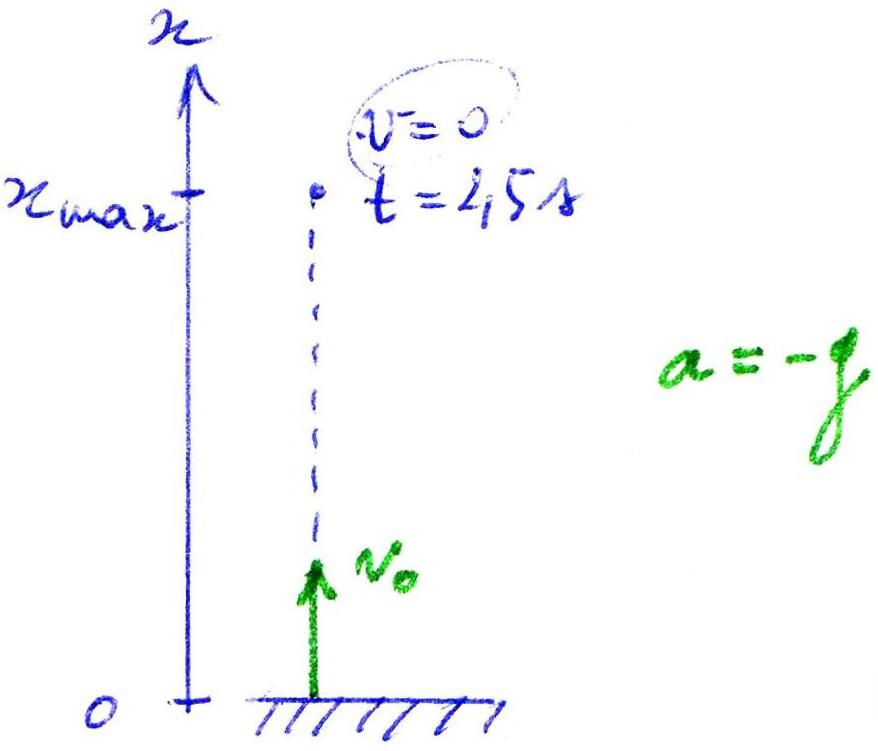
\includegraphics{55p44}
        \end{image}
        We krijgen:
        \begin{equation*}
            v=0\Leftrightarrow v_0-gt=0\Leftrightarrow v_0=gt
        \end{equation*}
        Dat is in grootte gelijk aan \SI{27}{m/s}. Nu dat we ook de beginsnelheid kennen, vinden we de afgelegde afstand, wat ook de maximale hoogte is:
        \begin{equation*}
            x=v_0t-\frac{1}{2}gt^2=(gt)t-\frac{1}{2}gt^2=\frac{1}{2}gt^2
        \end{equation*}
        Vullen we de getalwaardes in, dan vinden we \SI{38}{m}

        Merk op dat deze afstand gelijk is aan de afstand die de pijl vanuit rust zou afleggen bij een vrije val die \SI{2,8}{s} duurt. Dat is niet heel verwonderlijk; de vertraging naar boven toe is namelijk gelijk aan de versnelling bij het vallen naar beneden. Wiskundig loopt de symmetrieas van een parabool door de top. 
    \end{oplossing}
\end{exercise}

\begin{exercise}
    Een parachutist in vrije val bereikt een uiteindelijke valsnelheid van \SI{50}{m/s}. Neem aan dat een geopende parachute voor een constante vertraging van \SI{30}{m/s^2} zorgt.\footnote{Dit is een heel ruwe benadering. In feite hangt de vertraging door de parachute namelijk af van de snelheid en is die afhankelijkheid bovendien voor grote snelheden sterker dan voor kleine.} Wil er bij het neerkomen geen kans op letsel bestaan, dan mag de landingssnelheid niet groter dan \SI{5,0}{m/s} zijn.

    Wat is de minimumhoogte voor het openen van de parachute?
    \begin{oplossing}
        Aangezien we de versnelling en begin- en eindsnelheid kennen, kunnen we de tijd die nodig is om de eindsnelheid te bereiken, berekenen:
        \begin{eqnarray*}
            v=v_0+at&\Leftrightarrow&t=\frac{v-v_0}{a}
        \end{eqnarray*}
        De afgelegde afstand is dan met de gemiddelde snelheid te berekenen:
        \begin{eqnarray*}
            x&=&\overline{v}t\\
            &=&\frac{v_0+v}{2}\cdot\frac{v-v_0}{a}\\
            &=&\frac{v^2-v_0^2}{2a}\\
            &=&\SI{41,25}{m}
        \end{eqnarray*}
    \end{oplossing}
\end{exercise}

\begin{exercise}
    Iemand laat een meloen vallen vanop een hoogte van \SI{20}{m}. Op hetzelfde moment schiet je een pijl verticaal omhoog vanop de grond. De pijl treft de meloen na \SI{1,0}{s}. 
    \begin{enumerate}
        \item Geef in \'e\'en assenstelsel een verzorgde schets van de grafiek van de plaats in functie van de tijd voor beide objecten.
        \item Met welke snelheid heb je de pijl afgeschoten? 
    \end{enumerate}
    \begin{oplossing}
        De plaatsfunctie van de meloen gelijkstellen aan die van de afgeschoten pijl, geeft (we kiezen de $y$-as omhoog waardoor de versnelling de negatieve valversnelling is):
        \begin{eqnarray*}
           y_0-\frac{1}{2}gt^2&=&v_0t-\frac{1}{2}gt^2
        \end{eqnarray*}
        Oplossen naar $v_0$ geeft: $v_0=\frac{y_0}{t}=\SI{20}{m/s}$.
    \end{oplossing}
\end{exercise}

\begin{exercise}
    ($\ast\ast\ast$) Wanneer de pelikaan naar vis duikt, trekt hij zijn vleugels in om als een steen loodrecht naar beneden te vallen.

    Stel een pelikaan duikt vanaf \SI{25}{m} hoogte en verandert onderweg dus niet meer van koers. Als het een vis \SI{0,15}{s} kost om te vluchten, wat is dan de hoogte waarop de vis de pelikaan minstens moet opmerken, wil de vis nog kans maken te ontsnappen?

    Neem aan dat de vis zich aan het wateroppervlak bevindt.

    \begin{oplossing}
        We kiezen de referentie-as naar beneden, met de oorsprong op de positie waar de pelikaan begint aan zijn duik De versnelling is dan gelijk aan de valversnelling. 

        We kennen de afstand waarover de pelikaan valt zodat we de tijd die de pelikaan nodig heeft om het wateroppervlak te bereiken, de valtijd, kunnen berekenen uit $x_2=\frac{1}{2}gt_2^2 $:
        \begin{eqnarray*}
            t_2=\sqrt{\frac{2x_2}{g}}
        \end{eqnarray*}
        De pelikaan heeft namelijk geen beginsnelheid.

        Gedurende een tijd $t_1=t_2-\Delta t$ (15 honderdste van een seconde minder dan de valtijd) mag de pelikaan vallen zonder door de vis te worden opgemerkt. De afstand boven het wateroppervlak is dan:
        \begin{eqnarray*}
            x_2-x_1&=&x_2-\frac{1}{2}gt_1^2\\
            &=&x_2-\frac{1}{2}g\left(t_2-\Delta t\right)^2\\
            %&=&x_2-\frac{1}{2}g\left(\sqrt{\frac{2x_2}{g}}-\Delta t\right)^2\\
            %&=&\Delta t\sqrt{2gx_2}-\frac{1}{2}g\Delta t^2\\
            &=&\SI{3,2}{m}
        \end{eqnarray*}
    \end{oplossing} 
\end{exercise}

\begin{exercise}
    ($\ast\ast\ast$) Een verticaal vallende steen legt in de laatste seconde, voor hij de grond bereikt, \SI{100}{m} af. Men veronderstelt dat hij vanuit rust vertrok.
    \begin{enumerate}
        \item Bepaal de snelheid op het ogenblik dat hij de grond bereikt.
        \item Bepaal de hoogte vanwaar de steen viel en de tijd die hij daarvoor nodig had.
    \end{enumerate}

    \begin{oplossing}
        We kiezen de $x$-as naar beneden zodat de versnelling de valversnelling is, $a=g$. Als we $x_1$ beschouwen als de beginpositie van de beweging die de steen uitvoert in de laatste honderd meter, kunnen we de snelheid vinden waarmee de steen hieraan `begint'.
        \begin{eqnarray*}
            &&\Delta x=v_1\Delta t+\frac{1}{2}g\Delta t^2\\
            &\Leftrightarrow&v_1=\frac{\Delta x-\frac{1}{2}g\Delta t^2}{\Delta t}
        \end{eqnarray*}
        \begin{image}
            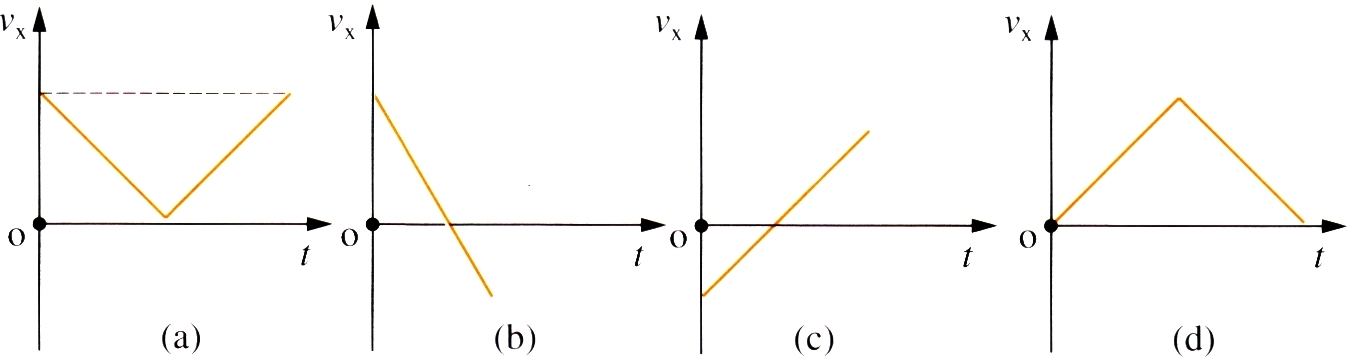
\includegraphics{valbeweging}
        \end{image}
        Met de formule voor de snelheid van een EVRB, vinden we de snelheid op het einde van het interval.
        \begin{eqnarray*}
            v_2&=&v_1+g\Delta t\\
            &=&\frac{\Delta x-\frac{1}{2}g\Delta t^2}{\Delta t}+g\Delta t\\
            &=&\cdots\\
            &=&\overline{v}+g\frac{\Delta t}{2}\\
            &=&\SI{105}{m/s}
        \end{eqnarray*}
        Je kan dit ook afleiden door gebruik te maken van de formule voor gemiddelde snelheid, $\overline{v}=\frac{v_1+v_2}{2}$.
        
        Omdat we de snelheid kennen, kunnen we de tijd vinden die de steen nodig heeft gehad om aan deze snelheid te komen. Vervolgens vinden we dan ook de afstand.
        \begin{eqnarray*}
            t_2=\frac{v_2}{g}=\frac{\overline{v}}{g}+\frac{\Delta t}{2}=\SI{10,7}{s}\\
            x_2=\frac{1}{2}gt_2^2=\SI{561}{m}
        \end{eqnarray*}
    \end{oplossing}
\end{exercise}

\begin{exercise}
    ($\ast\ast\ast$) Van de Empire Stage Building in New York komt op \SI{250}{m} een ijskegel los en valt naar beneden.
    \begin{enumerate}
        \item Na hoeveel tijd en met welke snelheid bereikt het ijskegeltje uiteindelijk de grond?
        \item Hoelang en over welke afstand moet de ijskegel al gevallen zijn om in de daaropvolgende \SI{2}{s} een afstand te kunnen afleggen van \SI{100}{m}?
    \end{enumerate}
    \begin{oplossing}
        \begin{enumerate}
            \item[Gegeven]$x_3=\SI{250}{m}$\newline$\Delta t=t_2-t_1=\SI{2,0}{s}$\newline$\Delta x=x_2-x_1=\SI{100}{m}$
            \item[Gevraagd]$t_3,v_3,t_1$ en $x_1$
        \end{enumerate}

        Omdat de beweging enkel naar beneden is, is de beschrijving gemakkelijk met een $x$-as naar beneden gericht. De versnellingscomponent $a$ is dan gelijk aan de valversnelling $g$. Omdat de kegel vanuit rust vertrekt, vinden we de valtijd uit $x=\frac{1}{2}gt^2$:
        \begin{equation*}   
            t=\sqrt{\frac{2x}{g}}
        \end{equation*}
        De valtijd bepaalt de eindsnelheid:
        \begin{equation*}
            v=gt=g\sqrt{\frac{2x}{g}}=\sqrt{2gx}
        \end{equation*}
        \begin{image}
            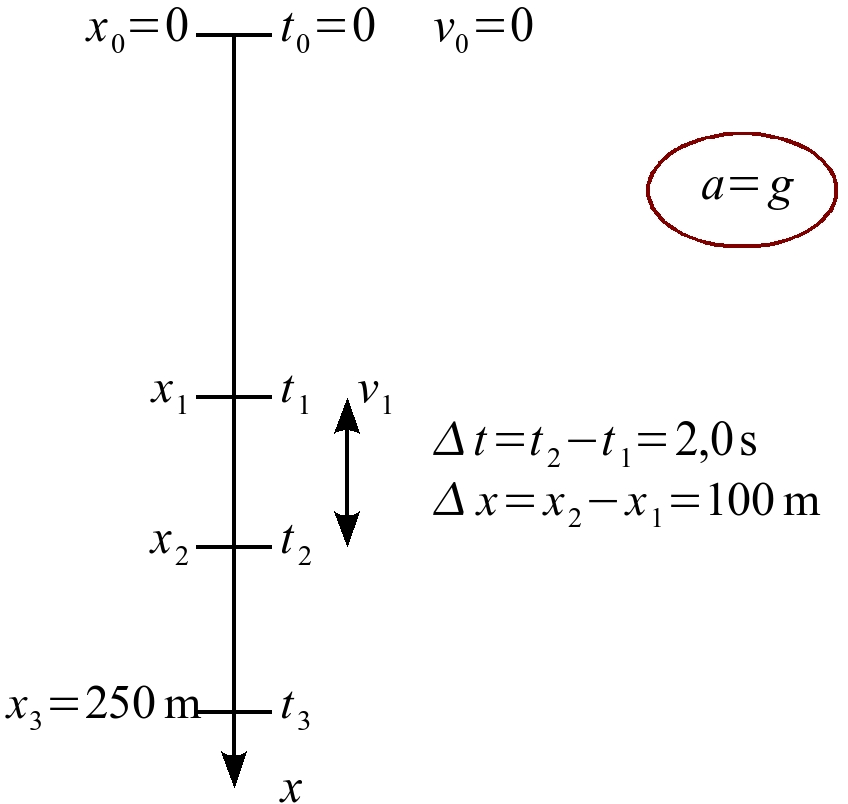
\includegraphics{opdr16p28}
        \end{image}
        Invullen van de gegevens geeft $t_3=\SI{7,1}{s}$ en $v_3=\SI{70}{m/s}=\SI{252}{km/h}$.

        Uit de plaatsfunctie kunnen we de beginsnelheid\footnote{Voor de honderd meter is de beginsnelheid $v_1$.} halen. De beginsnelheid $v_1$ is immers de enige onbekende in de vergelijking:\footnote{Hoe komen we aan deze uitdrukking? De plaatsfunctie toegepast op de honderd meter geeft: $x_2=x_1+v_1t+\frac{1}{2}gt^2$ waarin de variabele $t$ de verstreken tijd tussen tussen de posities $x_1$ en $x_2$ weergeeft. In dit geval stellen we die echter voor door $\Delta t$. Ook is $\Delta x=x_2-x_1$.}
        \begin{equation*}
            \Delta x=v_1\Delta t+\frac{1}{2}g\Delta t^2\\
        \end{equation*}
        Dus: $v_1=\frac{2\Delta x-g\Delta t^2}{2\Delta t}$.\footnote{Als we de uitdrukking uitwerken: $v_1=\frac{2\Delta x-g\Delta t^2}{2\Delta t}=\frac{\Delta x}{\Delta t}-g\frac{\Delta t}{2}=\bar{v}-g\frac{\Delta t}{2}$, is te zien dat $v_1$ \'e\'en seconde eerder dan de gemiddelde snelheid bereikt wordt. De gemiddelde snelheid is immers $\bar{v}=\frac{v_1+v_2}{2}$ en wordt dus halverwege de valtijd van de honderd meter bereikt. Bovendien toont deze uitwerking dat we het vraagstuk ook anders hadden kunnen oplossen. Uit $\frac{\Delta x}{\Delta t}=\frac{v_1+v_2}{2}=\frac{v_1+(v_1+g\Delta t)}{2}$ is immers $v_1$ te bepalen.}
        
        Omdat de kegel vanuit rust begint te vallen en per seconde \SI{9,81}{m/s} sneller valt, vinden we de valtijd als $t_1=\frac{v_1}{g}$:
        \begin{eqnarray*}
            t_1=\frac{2\Delta x-g\Delta t^2}{2g\Delta t}&=&\frac{2\cdot100\rm\,m-9,81\rm\,m/s^2\cdot(2,0\rm\,s)^2}{2\cdot9,81\rm\,m/s^2\cdot2,0\rm\,s}=\SI{4,1}{s}
        \end{eqnarray*}
        De bijbehorende afgelegde weg is dan $x_1=\frac{1}{2}gt_1^2=\SI{82}{m}$.
    \end{oplossing}
\end{exercise}
% Bron Fysica Vandaag 2 p. 92

\begin{exercise}
    ($\ast\ast\ast$) Een ziek man zit voor een raam dat \SI{1,20}{m} hoog is. Een steen wordt vanop de grond opgeworpen en passeert het raam een keer opwaarts en een keer neerwaarts. De man ziet de steen in totaal voor \'e\'en seconde.% (Een halve bij het opgaan en een halve bij het terug naar beneden gaan.)
    \begin{enumerate}
        \item Bepaal de snelheid waarmee de steen de onderkant van het raam bereikt.% (die is op het teken na hetzelfde in zowel de opwaartse als de neerwaartse beweging).
        \item Toon aan dat het met deze gegevens niet mogelijk is te berekenen hoe hoog het raam boven de grond is gelegen.
    \end{enumerate}
    \begin{oplossing}
        (a) $\Delta x= v_1\Delta t-\frac{1}{2}g\Delta t^2$ zodat $v_1=\bar{v}+g\frac{\Delta t}{2}=\SI{4,85}{m/s}$ ($\Delta t = \SI{0,5}{s}$)
        
        (b) Naast de hoogte van het raam boven de grond, zijn ook de benodigde tijd en de beginsnelheid onbekende grootheden. Met maar twee vergelijkingen die een EVRB beschrijven ($x=x_0+v_0t+\frac{1}{2}at^2$ en $v=v_0+at$), zijn deze onbekenden niet vast te leggen. 
        
        In een meer fysische uitleg kan je je realiseren dat eenzelfde snelheid aan de onderkant van het raam voor een grotere hoogte boven de grond te realiseren is met een grotere snelheid waarmee de steen opgeworpen wordt.
    \end{oplossing}
\end{exercise}
% Bron Herman Van Bouwel

\begin{exercise}
    ($\ast\ast\ast$) Een student gooit een sleutelbos verticaal omhoog naar een medebewoonster in een raam \SI{4,00}{m} hoger. De sleutels worden \SI{1,50}{s} later opgevangen.
    \begin{enumerate}
        \item Wat was de snelheid waarmee de sleutels omhoog werden gegooid?
        \item Welke snelheid had de sleutelbos vlak voordat hij werd opgevangen?
    \end{enumerate}
    \begin{oplossing}
        $v_0=\frac{x+\frac{1}{2}gt^2}{t}=10,02\rm\,m/s$ 

        $v=v_0-gt=\frac{x}{t}-\frac{1}{2}gt=\SI{-4,69}{m/s}$

        Merk op dat de sleutelbos wordt opgevangen bij het terug naar beneden komen. De snelheidscomponent is immers negatief.
    \end{oplossing}
\end{exercise}
% Bron Herman Van Bouwel

\begin{exercise}
    ($\ast\ast\ast$) Een voorwerp wordt verticaal omhoog geworpen en bereikt na een tijd $t$ een hoogte $h$. Toon aan dat de maximale hoogte $h_{\text{max}}$ die het voorwerp bereikt, wordt gegeven door:
    \begin{eqnarray*}
        h_{\text{max}}&=&\frac{(gt^2+2h)^2}{8gt^2}.
    \end{eqnarray*}
    \begin{oplossing}
        We zoeken eerst een uitdrukking voor de maximale hoogte. Op het hoogste punt is de snelheid nul zodat:
        \begin{eqnarray*}
            v&=&0\\
            &\Updownarrow&\\
            v_0-gt&=&0\\
            &\Updownarrow&\\
            t&=&\frac{v_0}{g}
        \end{eqnarray*}
        Deze tijd is dus de tijd die het voorwerp nodig heeft om het hoogste punt te bereiken. Als we de oorsprong van de $y$-as op de grond kiezen en naar boven gericht, dan vinden we de maximale hoogte door dit tijdstip in de plaatsfunctie in te vullen:
        \begin{eqnarray*}
            y_{max}&=&y(t_{max})\\
            &=&v_0\cdot\left(\frac{v_0}{g}\right)-\frac{1}{2}g\left(\frac{v_0}{g}\right)^2\\
            &=&\frac{v_0^2}{2g}
        \end{eqnarray*}
        Doordat we weten hoe hoog het voorwerp zich bevindt na een tijd $t_1$, kunnen we de beginsnelheid $v_0$ bepalen:
        \begin{eqnarray*}
            y_1&=&v_0t_1-\frac{1}{2}gt_1^2\\
            &\Updownarrow&\\
            v_0&=&\frac{2y_1+gt_1^2}{2t_1}
        \end{eqnarray*}
        Substitutie hiervan in de uitdrukking voor de maximale hoogte geeft de te bewijzen uitdrukking.
    \end{oplossing}
\end{exercise}

\end{document}
